\section{Visualizing directed comparative distributions}\label{sec:ComparativeDirected}

\subsection{Sankey diagrams and translation graphs}\label{ref:SankeyPlots}

One of the simplest ways of representing translation choices
visually is by using Sankey diagrams, named after H.R. Sankey
\citep{KennedySankey1898}. Figure \ref{fig:SankeyDeFr} (generated with
the package \verb+networkD3+ for \verb+R+, cf.
\citealt{networkD3-package}) shows a Sankey plot visualizing
the frequencies of (French) target language choices for the two German
source language expressions \textit{gleich} and
\textit{sofort}.\footnote{In Pyhon, the \verb+plotly+ module can be
  used to create Sankey diagrams.}

\begin{figure}[t]
  \centering
  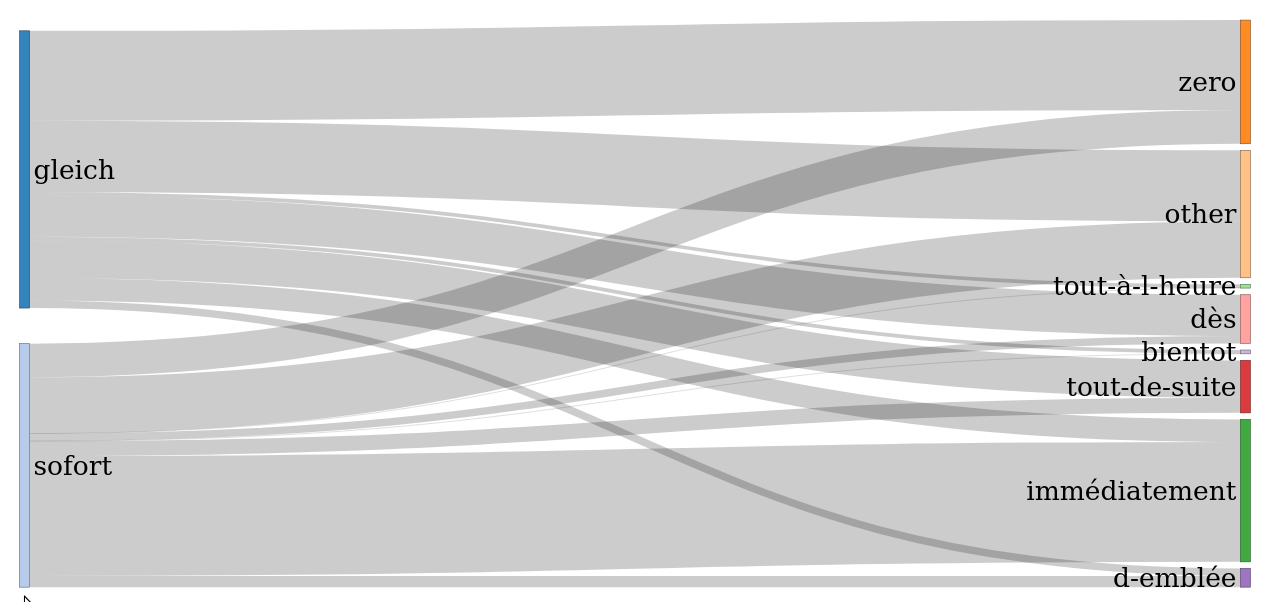
\includegraphics[width=0.85\linewidth]{figures/Sankey-de-fr.png}
  \cprotect\caption{Sankey plot showing French translations of the German
    \ipadv s \textit{gleich} and \textit{sofort}. The plot was
    generated with the package \verb+networkD3+ for \verb+R+
    \citep{networkD3-package}.}
  \label{fig:SankeyDeFr}
\end{figure}

We can add more information to `plain' Sankey diagrams by including an
intermediate layer of nodes displaying the frequencies of the levels of
some variable relative the source and target expressions, as in Figure
\ref{fig:SankeyDeFrRef}. The plot shows the frequencies of source and target
language correspondences mediated by the variable \textsc{Reference
point}. We can see that most cases of `deic[tic]-dir[ect]' come
from \textit{gleich} and go to `zero' or `other' (in French), while
almost all cases of `deic[tic]-phant[asma]' come from \textit{sofort}
and go to \textit{immédiatement}. Cases of `chron[ological]-ev[ent]'
seem to be typically associated with \textit{sofort} in German
originals, and with \textit{immédiatement} in French translations.

\begin{figure}[t]
  \centering
  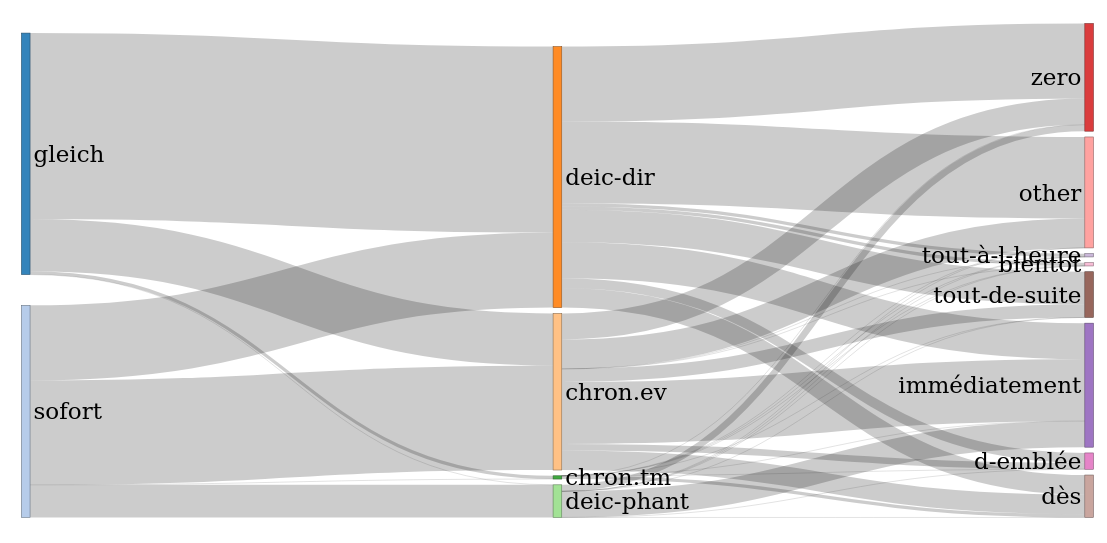
\includegraphics[width=0.9\linewidth]{figures/Sankey-de-fr-ref.png}
  \cprotect\caption{Comparative Sankey plot showing associations of
    IP-adverbials with French IP-adverbials, given the value for the
    variable \textsc{Reference point}. The plot was generated with the package
    \verb+networkD3+ for \verb+R+ \citep{networkD3-package}.}
  \label{fig:SankeyDeFrRef}
\end{figure}

To obtain a more global view, consider Figure
\ref{fig:SankeyDeFrCluster}, which shows the correspondences between
source and target language expressions relative to the clusters
mentioned in Sect. \ref{sec:ComparativeUndirected} (solution with
three clusters). We already know that Cluster 1 is positively associated
with \textit{gleich} in German. The plot shows that most cases of this
category go to `zero' or `other' in French. Clusters 2 and 3 are
more evenly distributed among \textit{gleich} and \textit{sofort} in
German, but they also seem to exhibit clear asymmetries.

While Sankey plots contain useful (relational) information about
frequency distributions in the source and target language, they do not
contain by-item information and are potentially deceptive. The edges
conecting the nodes reflect frequencies, but the left edges are not
connected by-item to the right edges. For example, as mentioned above,
if we look at the middle node `chron.ev' (for `chronological relative
to an event'), the plot suggests that those cases that are rendered
with \textit{gleich} in German go to `zero' and `other' in
French. While this is probably true, the underlying data does not
actually contain that information. Like a CA, Sankey diagrams are
built on cross-tables and merely represent frequencies of combinations
of levels for pairs of crossed variables. For example, it would be
conceivable that most or even all occurrences of \textit{sofort} going
to `deic-dir' actually end up at `zero'.

\begin{figure}[t]
  \centering
  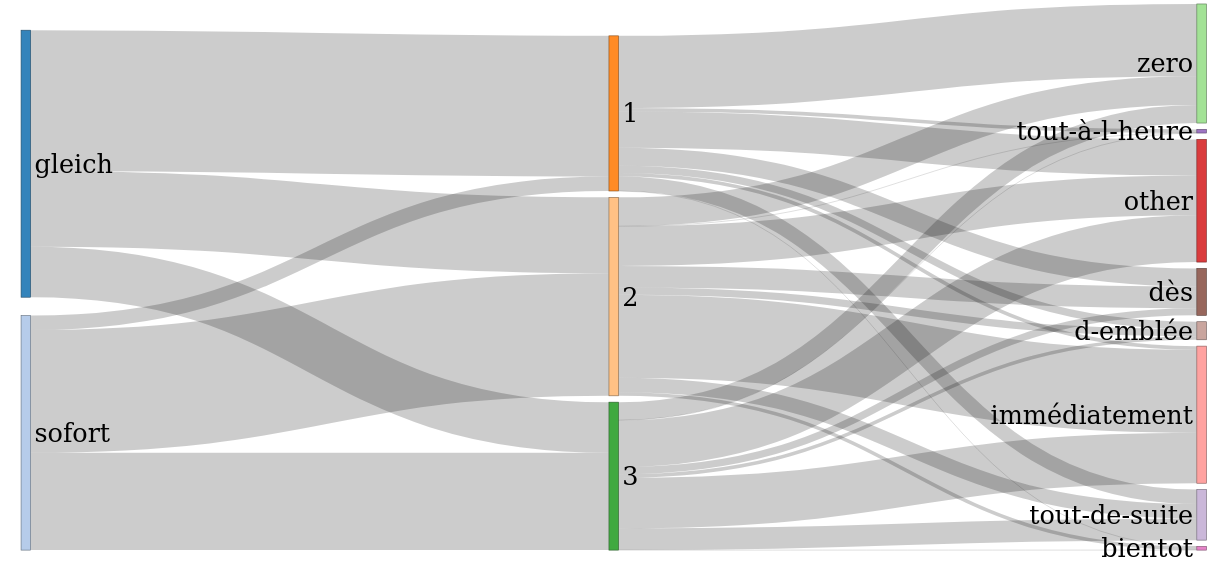
\includegraphics[width=0.9\linewidth]{figures/Sankey-de-fr-pam-low.png}
  \cprotect\caption{Comparative Sankey plot showing associations of
    IP-adverbials with French IP-adverbials, given a specific context
    cluster (solution with three clusters). The plot was generated with
    the package \verb+networkD3+ for \verb+R+
    \citep{networkD3-package}.}
  \label{fig:SankeyDeFrCluster}
\end{figure}


Translation choices can be represented more precisely with
visualizations that we call Context-Conditional Translation Graphs (CCTG; see also
\citealt{GastAtayan2019}). Consider the graph in Figure
\ref{fig:NetworkDeFr}.  It shows frequencies of choices made in
German-to-French translation, under specific contextual
conditions. The colours of the edges correspond to the three clusters
of context variables (see also the caption of the graph).
%
Figure \ref{fig:NetworkDeFr} shows that \textit{gleich} is indeed
mostly not translated at all in Context 1. \textit{Sofort} typically
goes to \textit{immédiatement} in Contexts 2 and 3. Unlike suggested
by Figure \ref{fig:SankeyDeFrCluster}, there does not seem to be any
particular association between \textit{gleich} and `other', as the
three arrows between these nodes have approximately the same width.

\begin{figure}[t]
  \centering
  % 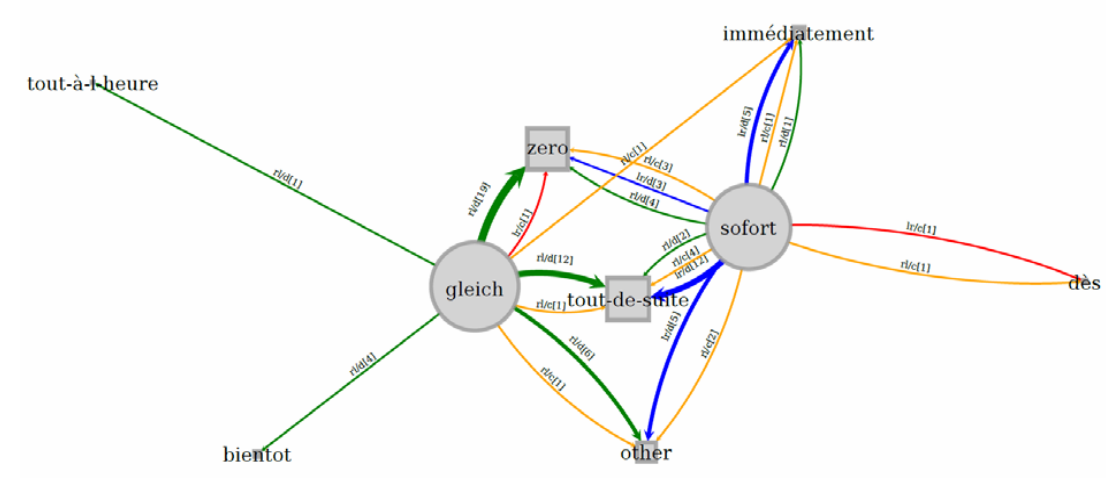
\includegraphics[width=\linewidth]{figures/TranslationGraphDeFr.png}
  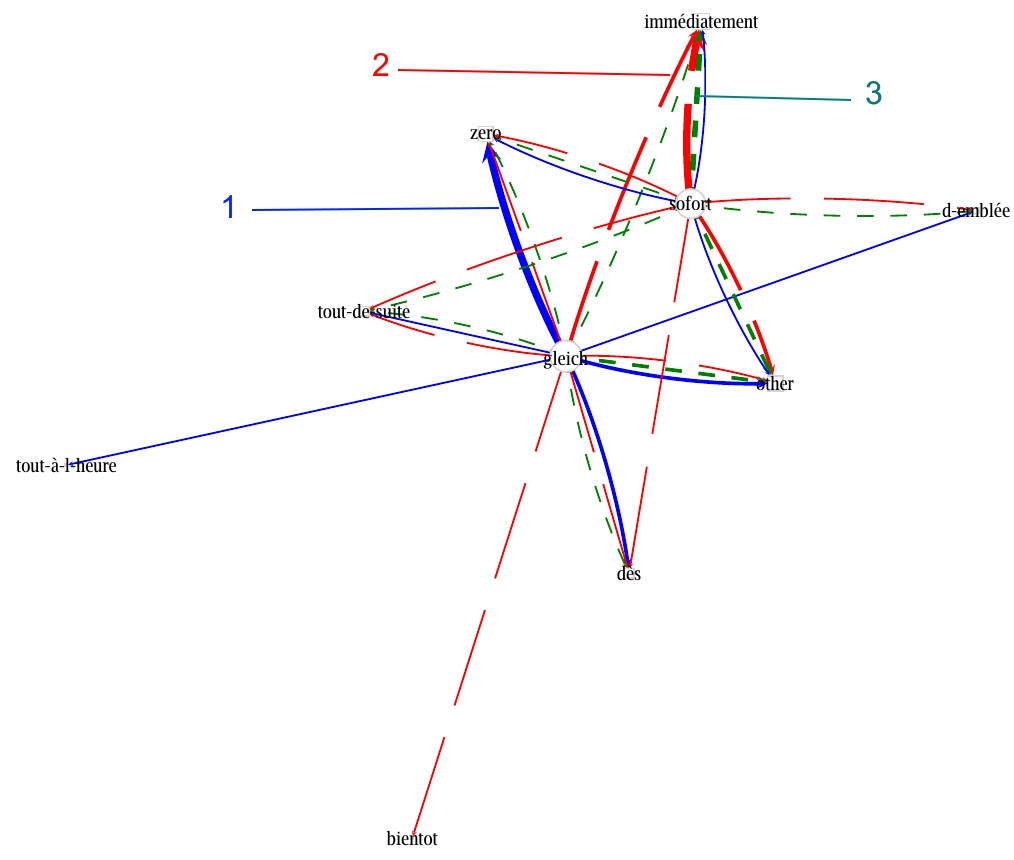
\includegraphics[width=\linewidth]{figures/network-de-fr.jpg}
  \cprotect\caption{Context-Conditional Translation Graph showing French
    translation choices for German \textit{gleich} and
    \textit{sofort}, given specific context clusters. The (solid) blue
    edge indicates translation in Context 1, the (long-dashed) red
    line represents translations in Context 2, and the (short-dashed)
    green line corresponds to Context 3. The graph was generated with
    the package \verb+graph_tool+ for \verb+Python+
    (https://graph-tool.skewed.de/static/doc/); see the script \verb+IpNetwork.py+ in the Supplementary Materials.}
  \label{fig:NetworkDeFr}
\end{figure}

%Once again, we wish to emphasize that impressions based on visualizations like the one in Figure \ref{fig:NetworkDeFr} should of course be supported by statistical evidence. 
%We will now sketch out ways of handling translation data using methods from Bayesian statistics.





%%% Local Variables:
%%% mode: latex
%%% TeX-master: "main"
%%% End:

